\documentclass{standalone}

\usepackage{tikz}
\usepackage{circuitikz}

\tikzset{block/.style = {draw, fill=white, very thick, rectangle, minimum height=1cm, minimum width=2cm},
         lblock/.style={draw,fill=white,very thick, rectangle, minimum height=3cm, minimum width=1cm},
         sum/.style= {draw, fill=white, very thick, circle, node distance=0.5cm}}

         
\begin{document}
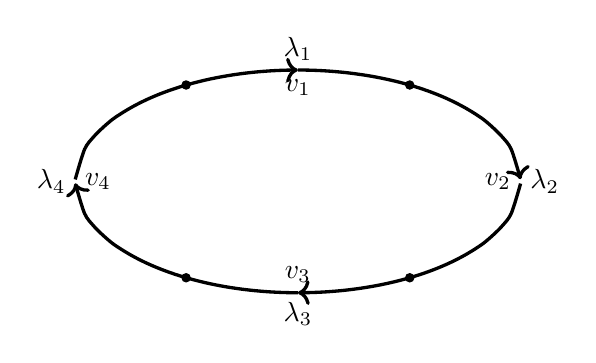
\begin{tikzpicture}[scale=2]
    \draw[->,very thick]plot[smooth, domain=0:1.414](\x,{(0.5-(1/2*\x)^2)^0.5});
    \draw[->,very thick]plot[smooth, domain=-1.414:0](\x,{(0.5-(1/2*\x)^2)^0.5});
    \draw[<-,very thick]plot[smooth, domain=0:1.414](\x,{-(0.5-(1/2*\x)^2)^0.5});
    \draw[<-,very thick]plot[smooth, domain=-1.414:0](\x,{-(0.5-(1/2*\x)^2)^0.5});


    \filldraw[black](0.71,0.612)circle(0.75pt);
    \node[above]at(0,0.707){$\lambda_1$};
    \node[below]at(0,0.707){$v_1$};

    \filldraw[black](0.71,-0.612)circle(0.75pt);
    \node[below]at(0,-0.707){$\lambda_3$};
    \node[above]at(0,-0.707){$v_3$};

    \filldraw[black](-0.71,0.612)circle(0.75pt);
    \node[right]at(1.414,0){$\lambda_2$};
    \node[left]at(1.414,0){$v_2$};

    \filldraw[black](-0.71,-0.612)circle(0.75pt);
    \node[left]at(-1.414,0){$\lambda_4$};
    \node[right]at(-1.414,0){$v_4$};
\end{tikzpicture}
\end{document}